\chapter{集合与映射}
\label{chp:Set-list-map}

\section*{基本信息}
\sline
\begin{description}
\item[课程名称:] Java应用与开发
\item[授课教师:] 王晓东
\item[授课时间:] 第五周;第六周
\item[参考教材:] 本课程参考教材及资料如下:
  \begin{itemize}
  \item 陈国君主编,Java程序设计基础(第5版),清华大学出版社,2015.5
  \item Bruce Eckel, Thinking in Java (3rd)
  \end{itemize}
\end{description}

\section*{教学目标}

\sline

\begin{enumerate}
\item 掌握列表(List)、集(Set)、映射(Map)的概念、层次关系及应用
\item 掌握迭代器(iterator)、Enumeration接口等容器操作常用API
\end{enumerate}

\section*{授课方式}

\sline
\begin{description}
\item[理论课:] 多媒体教学、程序演示
\item[实验课:] 上机编程
\end{description}

\newpage
\section*{教学内容}
\sline

\section{集合概念及分类}


\subsection{集合和数组}


在编程中,常常需要集中存放多个数据。从传统意义上讲,数组是我们的一个很
好的选择,前提是我们事先已经明确知道我们将要保存的对象的数量。一旦在数
组初始化时指定了这个数组长度,这个数组长度就是不可变的。如果我们需要保
存一个可以动态增长的数据(在编译时无法确定具体的数量),java的集合类就
是一个很好的设计方案了。

面向存放多个数据的需求,数组和集合类型具有以下用法差异:
  
\begin{itemize}
\item 数组用于存放指定长度的数据。
\item 需要保存可以动态增长的数据(在编译时无法确定具体的
  数量),则需要用到Java的集合类。
\end{itemize}

\subsection{集合类型}

{\hei\Red 集合就是将若干用途、性质相同或相近的“数据”组合而成一个整体。}集合类型分类如下:

\begin{description}
\item[集] Set集合中不区分元素的顺序,不允许出现重复元素。例如应用于记
  录所有用户名的场合。
\item[列表] List集合区分元素的顺序,且允许包含重复元素。相当于数据结
  构中的线性表,具体表现为数组和向量、链表、栈、队列等。
\item[映射] Map中保存成对的“键\ding{213}值”(Key-Value)信息,映射中不能包含重
  复的键,每个键最多只能映射一个值。
\end{description}


\notice{注意}
  
{\kai Java集合中只能保存引用类型的数据,实际上存放的是对象的引用而非对
  象本身。Java API中的集合类型均定义在java.util包中。}

\subsection{对Java集合中只能保存引用类型的数据的说明}

Java集合只能存放引用类型数据,它们都是存放引用类型数据的容器,不能存
放如int、long、float、double等基本类型的数据。

\subsubsection{集合存储对象}

Java集合中实际存放的只是对象的引用,每个集合元素都是一个引用变量,实
际内容都放在堆内存或者方法区里面,但是基本数据类型是在栈内存上分配空
间的,栈上的数据随时就会被收回的。

\subsubsection{基本类型数据如何解决呢?}

可以通过包装类把基本类型转为对象类型,存放引用就可以解决这个问题。更
方便的,由于有了自动拆箱和装箱功能,基本数据类型和其对应对象(包装类)
之间的转换变得很方便,想把基本数据类型存入集合中,直接存就可以了,系
统会自动将其装箱成封装类,然后加入到集合当中。

\subsection{集合相关API的关系}

\begin{figure}[htb]
\centering
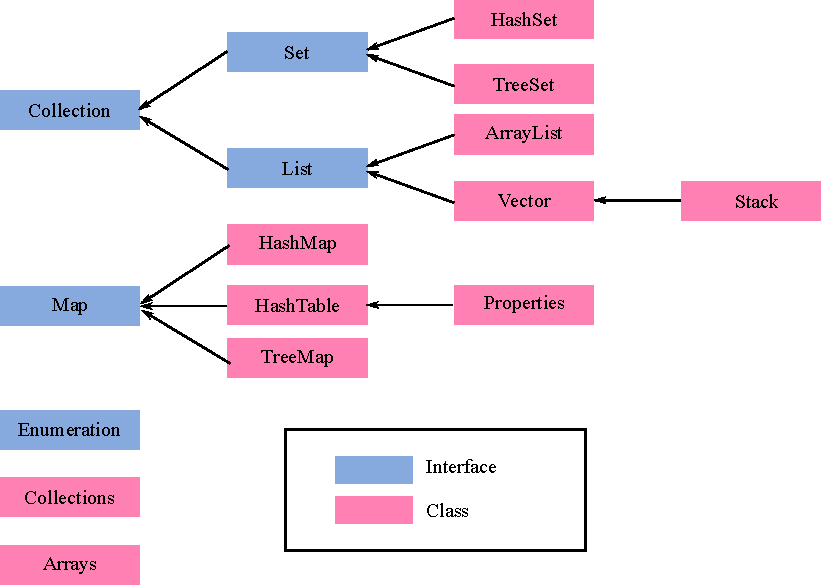
\includegraphics[width=\textwidth]{images/Set-list-map/fig-set-list-map.pdf}
\caption{集合相关API的关系}
\label{fig:set-map-list}
\end{figure}

\section{Collection和Map接口}

\subsection{Collection接口}

java.util.Collection接口是描述Set和List集合类型(不包含Map)的根接口,
其中定义了有关集合操作的普遍性方法:
  
\begin{itemize}
\item boolean add(Object o) 向集合中添加一个元素,在子接口中此方法发生
  了分化,如Set接口中添加重复元素时会被拒绝(返回false,而不是出错
  );List接口则会接受重复元素且返回true。
\item boolean remove(Object o) 从集合中移除指定的元素。
\item int size() 返回集合中元素的数目。
\item boolean isEmpty() 判断集合是否为空(即是否包含任何元素)。
\item boolean contains(Object o) 判断集合中是否包含指定的元素。
\item void clear() 移除当前集合中的所有元素。
\item Iterator iterator() 返回在此集合的元素上进行迭代的迭代器。
\item Object[] toArray() 返回包含当前集合中所有元素的数组。
\end{itemize}


\subsection{Set和List接口}

java.util.Set和java.util.List分别描述前述的集和列表结构,二者均
为Collection的子接口。

Set接口模拟了数学意义的集合。List接口规定使用者可以对列表元素的插入位置
进行精确控制,并添加了根据元素索引来访问元素等功能,接口中新添加了相应
方法:

\begin{itemize}
\item void add(int index, Object element)
\item Object get(int index)
\item Object set(int index, Object element) 
\item int indexOf(Object o) 返回列表中首次出现指定元素的索引,如果列表不包含指定元素,则返回-1。
\item Object remove(int index)
\end{itemize}

\subsection{Map接口}

java.util.Map接口描述了映射结构,Map结构允许以{\hei\Blue 键集、值集合或
  键—值映射关系集}的形式查看某个映射的内容。主要方法:
  
\begin{itemize}
\item Object put(Object key, Object value) 向当前映射中加入一组新的
  健—值对,并返回所加入元素的“值”,如果此映射中以前包含一个该键的映射关
  系,则用新值替换旧值。
\item Object get(Object key) 返回此映射中映射到指定键的值,没有则返
  回null。
\item boolean isEmpty()
\item void clear()
\item int size()
\item boolean containsKey(Object key) 如果映射中包含指定键的映射关系,
  则返回true,否则返回false。
\item boolean containsValue(Object value)
\item Set keySet() 返回此映射中包含的键的set视图,此Set受映射支持,所以
  对映射的改变可以在此Set中反映出来,反之亦然。
\item Collection values()返回此映射包含值的Collection视图,
  此Collection受映射支持,所以对映射的改变可以在此Collection中反映出来,
  反之亦然。
\end{itemize}

\section{列表}

\subsection{ArrayList类}

java.util.ArrayList类实现了List接口,用于表述长度可变的数组列
表。ArrayList列表允许元素取值为null。除实现了List接口定义的所有功能外,
还提供了一些方法来操作列表容量的大小,相关方法包括:

\begin{itemize}
\item public ArrayList() 构造方法:创建一个初始容量为10的空列表。
\item public ArrayList(int initialCapacity)
\item {\Red public void ensureCapacity(int minCapacity) 对容器进行扩容。}
\item public void trimToSize() 将此ArrayList实例的容量调整为列表的当前大小。
\end{itemize}

\subsection{代码的局部性能优化 ensureCapacity}

合理的使用ArrayList ensureCapacity(int n)方法可以对代码性能进行优化:

\begin{itemize}
\item 该方法可以对ArrayList底层的数组进行扩容。
\item 显示的调用这个函数,如果参数大于低层数组长度的1.5倍,那么这个数
  组的容量就会被扩容到这个参数值,如果参数小于低层数组长度的1.5倍,那
  么这个容量就会被扩容到低层数组长度的1.5倍。
\item 在适当的时机,好好利用这个函数,将会使我们写出来的程序性能得到
  很大的提升。
\end{itemize}

\codeset{sample.setlistmap.ArrayListEnSureCapacitySample.java}


\subsection{Vector类}

java.util.Vector也实现了List接口,其描述的也是可变长度的对象数组。Vector与ArrayList的差别主要包括:

{\Red\kai Vector是同步(线程安全)的,运行效率要低一些,主要用在在多线
  程环境中,而ArrayList是不同步的,适合在单线程环境中使用。}

常用方法(除实现List接口中定义的方法外):

\begin{itemize}\small
\item public Vector()
\item public Object elementAt(int index)
\item public void addElement(Object obj)
\item public void removeElementAt(int index)
\item public void insertElementAt(E obj, int index) 
\item public boolean removeElement(Object obj) 
\item public void removeAllElements()
\item public Object[] toArray()
\end{itemize}


\subsection{什么是线程安全}

\begin{description}
\item[线程安全] 在多线程访问时采用加锁机制,当一个线程访问该类的某个
  数据时进行保护,其他线程不能进行访问直到该线程读取完,其他线程才可
  使用,不会出现数据不一致或者数据污染。(Vector、HashTable等)
\item[线程不安全] 不提供数据访问保护,有可能出现多个线程先后更改数据导致出现“脏数据”。
  (ArrayList、LinkedList、HashMap等)
\end{description}

\begin{figure}[htb]
\centering
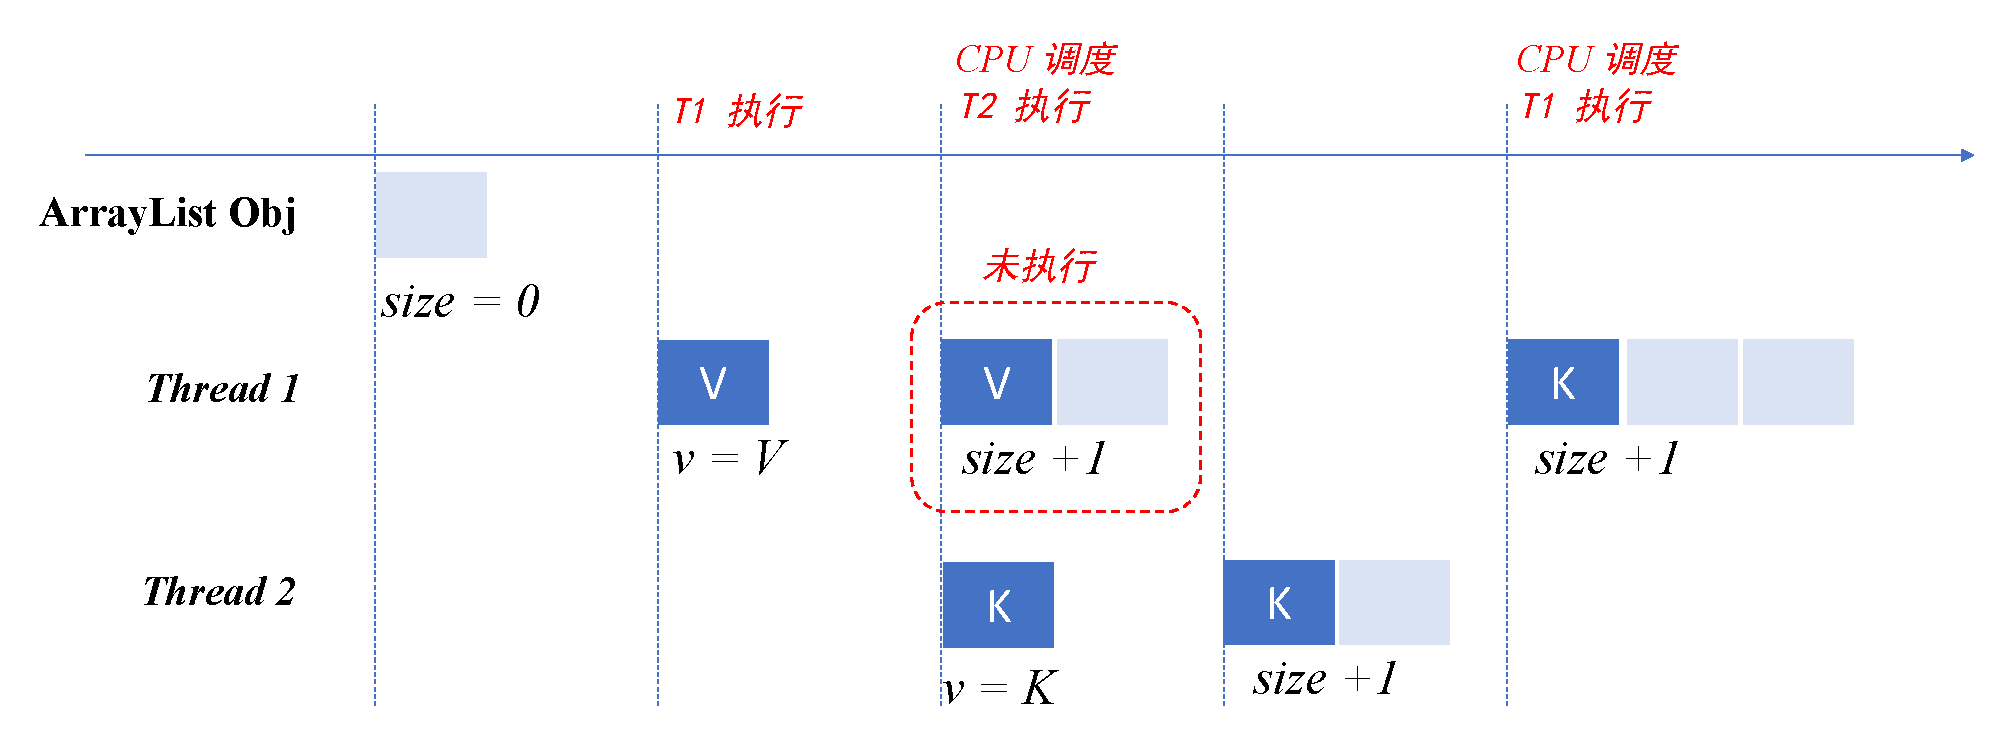
\includegraphics[width=\textwidth]{images/Set-list-map/thread-safe.pdf}
\caption{线程安全}
\label{fig:thread-safe}
\end{figure}

比如一个ArrayList类,在添加一个元素的时候,它可能会有两步来完成:

\begin{enumerate}
\item 在Items[Size]的位置存放此元素;
\item 增大Size的值。
\end{enumerate}

在单线程运行的情况下,如果Size=0,添加一个元素后,此元素在位置0,而
且Size=1; 而如果是在多线程情况下,比如有两个线程,线程A先将元素存放在
位置0。但是此时CPU调度线程A暂停,线程B得到运行的机会。线程B也向
此ArrayList添加元素,因为此时Size仍然等于0,所以线程B也将元素存放在位
置0。接下来线程A和线程B都继续运行,都增加Size的值。当前,ArrayList中元
素实际上只有一个,存放在位置0,而Size却等于2,这就是{\hei 线程不安全}。

\subsection{Stack}

java.util.Stack类继承了Vector类,对应数据结构中以{\hei\Blue “后进先
  出”(Last in First out, LIFO)方式存储和操作数据的对象栈}。Stack类提
供了常规的栈操作方法:

\begin{itemize}
\item public Stack() 构造方法,创建一个空栈。
\item public Object push(E item) 向栈中压入数据。
\item public Object pop() 移除栈顶对象并作为此方法的返回值。
\item public Object peek() 查看/返回栈顶对象,但不从栈中移除它。
\item public boolean empty() 测试栈是否为空。
\item public void clear() 清空栈。
\item public int search(Object o) 返回对象在栈中的位置,以1为基数。
\end{itemize}

\section{Iterator接口}

\subsection{Iterator接口概述}

\begin{itemize}
\item 对于ArrayList可以使用get()方法访问其元素;
\item 对于Vector,还可以使用elementAt()方法访问其元素;
\item 后续Set和Map集合也有各自不同的元素访问方式。
\end{itemize}

{\Blue\hei 是否有一种统一的方式来遍历各种不同类型集合中的元素呢?}

Java.util.Iterator接口描述的是以统一方式对各种集合元素进行遍历/迭代的工
具,也称为“{\Blue\hei 迭代器}”。迭代器允许在遍历过程中移除集合中的(当
前遍历到的那个)元素。主要方法包括:

\begin{itemize}
\item boolean hasNext() 如果仍有元素可以迭代,则返回true,否则返回false。
\item Object next() 返回迭代的下一个元素,重复调用此方法直到haseNext()方法返回false。
\item void remove() 将当前迭代到的元素从迭代器指向的集合中移除。
\end{itemize}

\subsection{使用迭代器}

我们一般不直接创建迭代器对象,而是通过调用集合对象的iterator()方法(该
方法在Collection接口中定义)来获取。

\samp{TestIterator.java}

\begin{javaCode}
  import java.util.ArrayList;
  import java.util.Iterator;

  public class TestIterator {
    public static void main(String[] args) {
      ArrayList a = new ArrayList();
      a.add("China");
      a.add("USA");
      a.add("Korea");
      Iterator it = a.iterator();
      
      while(it.hasNext()) {
        String country = (String) it.next();
        System.out.println(country);
      }
    }
  }
\end{javaCode}

\descript{注意}
迭代器相当于原始集合的一个“视图”,即一种表现形式,而不是复制其中所有元素得到的拷贝,因此在迭代器上的操作将影响到原来的集合。

\section{集}

\subsection{HashSet类}

java.util.HashSet类实现了java.util.Set接口,描述典型的Set集合结构。

\begin{itemize}
\item HashSet中不允许出现重复元素,不保证集合中元素的顺序。
\item HashSet中允许包含值为null的元素,但最多只能有一个null元素。
\end{itemize}

\subsection{TreeSet类}

java.util.TreeSet类也实现了java.util.Set,它描述的是Set的一种变体——可以
实现排序功能的集合。

\begin{itemize}
\item 在将对象元素添加到TreeSet集中时会自动按照某种比较规则将其插入到有
  序的对象序列中,以保证TreeSet集合元素组成的对象序列时刻按照“升序”排
  列(例如按照字典顺序排列);
\item 对于用户自定义的类型的数据可以自行定义其所需的排序规则(使用Comparable接口)。
\end{itemize}


\subsection{Comparable接口}

java.lang.Comparable接口中定义的compareTo()方法用于提供对其实现类的对象
进行整体排序所需的比较逻辑,所为的排序可以理解为按照某种标准来比较对象
的大小以确定其次序。

\begin{itemize}
\item 实现类基于compareTo()方法的排序被称为{\Blue 自然排序}。
\item compareTo()方法被称为它的{\Blue 自然比较方法},具体的排序原则可由
  实现类根据需要而定。
\end{itemize}

方法格式如下:

\begin{javaCode}
  int compareTo(Object o) {
  }   
\end{javaCode}


\subsubsection{使用Comparable接口实现自然排序}

\samp{Person.java}

\begin{javaCode}
  public class Person implements java.lang.Comparable {
    private final int id;
    ...

    public Person(int id, String name, int age) {
      this.id = id;
      ...
    }
    ...
    @Override
    public int compareTo(Object o) {
      Person p = (Person) o;
      return this.id - p.id;
    }
    @Override
    public boolean equals(Object o) {
      boolean flag = false;
      if (o instanceof Person) {
        if (this.id == ((Person) o).id) {
          flag = true;
        }
      }
      return flag;
    }
  } 
\end{javaCode}

\samp{TestComparable.java}

\begin{javaCode}
  import java.util.TreeSet;
  import java.util.Iterator;

  public class TestComparable {
    public static void main(String[] args) {
      TreeSet ts = new TreeSet();
      ts.add(new Person(1003, "Bob", 15));
      ts.add(new Person(1008, "Alice", 25));
      ts.add(new Person(1001, "Kevin", 30));
    }
    Iterator it = ts.iterator();
    while (it.hasNext()) {
      Person emplyee  = (Person) it.next();
      System.out.println(employee);
    }
  }
\end{javaCode}

\begin{stdoutCode}
  Id: 1001 Name: Kevin Age:30
  Id: 1003 Name: Bob Age:15
  Id: 1008 Name: Alice Age:25
\end{stdoutCode}

对上述程序的几点说明:

\begin{enumerate}
\item 用户在重写compareTo()方法以定制比较逻辑时,需要确保其与等价性判断
  方法equals()保持一致,即确保条件“{\Red (x.compareTo(y) == 0) ==
    (x.equals(y))}”永远成立,否则逻辑上不合理。所以上例同时重写
  了equals()方法。
\item 为保证能够实现元素的排序功能,TreeSet集合要求向其加入的对象元素必
  须是Comparable接口的实现类的实例,否者程序运行时会抛出{\Red 造型异
    常}(java.lang.ClassCastException)。
\item Comparable接口并不专用于集合框架。
\end{enumerate}

\section{映射}

\subsection{HashMap类}

java.util.HashMap类实现了java.util.Map接口,该类基于{\hei\Blue 哈希表}实现了前述的映射集合结构。

\begin{itemize}
\item HashMap结构不保证其中元素(映射信息)的先后顺序,且允许使用null“值”和null“键”。
\item 当集合中不存在当前检索的“键”所对应的映射值时,HashMap的get()方法会返回空值null,而不会运行出错。
\item 影响HashMap性能的两个参数:初始容量(Initial Capacity)和加载因子(Load Factor)。
\end{itemize}

\subsection{HashTable类}

java.util.Hashtable与HashMap作用基本相同,也实现了Map接口,采用哈希表的方式将“键”映射到相应的“值”。

Hashtable与HashMap的差别主要包含以下方面:

\begin{itemize}
\item Hashtable中元素的“键”和“值”均不允许为null,而HashMap则允许。
\item {\Red Hashtable是同步的,即线程安全的,效率相对要低一些,适合在多
    线程环境下使用;而 HashMap是不同步的,效率相对高一些,提倡在单线程
    环境中使用。}
\item 除此之外,Hashtable与HashMap的用法格式完全相同。
\end{itemize}

\subsection{TreeMap类}

java.util.TreeMap类实现了将Map映射中的元素按照“键”进行升序排列的功能,
其排序规则可以是默认的按照“键”的自然顺序排列,也可以使用指定的其他排序
规则。

向TreeMap映射中添加的元素“键”所属的类必须实现Comparable接口。

\begin{javaCode}
  public MyKey implements Comparable {
    private final int id;
    ...
    public MyKey(int id) {
      this.id = id;
    }
    ...
    @Override
    public int compareTo(Object o) {
      return this.id - ((MyKey) o).id;
    }
    @Override
    public boolean equals(Object o) {
      return (o instanceof MyKey) && (this.id == ((MyKey) o).id);
    }
    @Override
    public int hashCode() {
      return new Integer(id).hasCode();
    }
  }  
\end{javaCode}

\notice{对上述程序的说明}

{\kai MyKey类重写equals()方法的同时也重写了hasCode()方法,这是一种规
  范的做法,目的是为了维护hasCode()方法的常规协定,该协定要求相等对象
  必须具有相等的哈希码,即当两个对象使用equals()方法比较结果为等价时,
  它们各自调用hasCode()方法也应该返回相同的结果。}

\section{其他相关API}

\subsection{Enumeration接口}

java.util.Enumeration接口作用与Iterator接口类似,但只提供了遍
历Vector和Hashtable(及子类Properties)类型集合元素的功能,且不支持集合
元素的移除操作。

\begin{javaCode}
  import java.util.*;

  public class TestEnumeration {
    public static void main(String[] args) {
      Vector v = new Vector();
      v.addElement("Lisa");
      v.addElement("Billy");
      v.addElement("Brown");

      Enumeration e = v.elements();

      while(e.hasMoreElements()) {
        String value = (String) e.nextElement();
        System.out.println(value);
      }
    }
  }
\end{javaCode}

\subsection{Collections类}

java.util.Collections类定义了多种集合操作方法,能够实现了对集合元素
的{\Blue\hei 排序、取极值、批量拷贝、集合结构转换、循环移位以及匹配性检
  查}等功能。Collections类的主要方法包括:

\begin{itemize}\small
\item public static void sort(List list)
\item public static void reverse(List list)
\item public static void shuffle(List list)
\item public static void copy(List dest, List src)
\item public static ArrayList list(Enumeration e)
\item public static int frequency(Collection c, Object o)
\item public static T max(Collection coll)
\item public static T min(Collection coll)
\item public static void rotate(List list, int distance)
\end{itemize}

\subsection{Arrays类}

java.util.Arrays类定义了多种数组操作方法,实现了对数组元素的排序、填充、
转换为列表或字符串形式、增强的检索和深度比较等功能。Arrays类的主要方法
包括:

\begin{itemize}
\item public static List asList(Object... a)
\item public static void sort(<类型>[] a)
\item public static int binarySearch(int[] a, int key)
\item public static String toString(int[] a)
\end{itemize}

\notice{说明}

Arrays类在前面数组部分有阐述。


